\chapter{From signals to images}
\label{chapter:two}
%Contiene el método y el enfoque.

%Mental Chrometry and averaging 
%https://www.ncbi.nlm.nih.gov/pmc/articles/PMC548951/

This chapter describes the procedure to plot an image from the digital EEG signal.  This image is used to extract a feature which represents the waveform, the structure of the signal on a plot.  By analyzing this feature, we hypothesize that the underlying cognitive process can be detected and that it can be used to implement a brain-computer communication device.

\section{Electroencephalographic Plotting}

The plotting of the EEG is intrinsically mixed with the nuisances of the electroencephalography itself.  Plotting proceed by using a chart recorded with a single pen~\cite{Jestico1977}.   Voltages are represented on a vertical axis while time is represented on the horizontal axis, in a Cartesian arrangement. 

\begin{enumerate}
\item Sensitivity: also termed gain due the amplification procedure.  Its units are $ \frac{mV}{mm}$.  In the digital form, it is $\frac{\mu V}{pixel}$.
\item Epoch/Paper speed: the time span that is represented in a single screen.  For paper strips it was used to be $10s$ (Figure FIG).  In the digital version is $ \frac{\lambda}{pixel}$ with $\lambda$ being the length of the signal segment.
\end{enumerate}

On analog plotting montage was essential, but digital plotting allows to implement flexible configuration.  Montage can be monopolar or bipolar.  On Monopolar Montages each electrode obtain the potential difference against a common reference, and with Bipolar Montages, electrodes are paired, even in chained configurations, and the potential difference is obtained between them (cite Electroencphalograpy for empilepsy society).

%Logarithmic plotting, montage, calibration (cite Electroencphalograpy for empilepsy society)

\begin{story}[Neuroimaging]
With the advent of digital computers and the digital revolution, Plotting has become imaging.  Neuroimaging (CIte book Rodrigo Q Q) means mapping activity or structure to neuroanatomical regions (see Figure \ref{fig:neuroanatomy}).

There are currently three categories of neuroimaging: \textit{structural} includes CT (Computed Tomography), MRI (Magnetic Resonance Imaging) and DTI (Diffusion Tensor Imaging), \textit{functional}, which encompass EEG, MEG (Magnetoencephalography), fMRI (functional MRI) PET (Positron Emission Tomography), SPECT (Single Positron Emission Computed Tomography), NIRS (Near-Infrared Spectroscopy) and \textit{chemical} which involves dyes which are sensible to neuron firing.
\end{story}

\section{Signal to Image transformation}

The EEG signal may be represented by

\begin{equation}
\mathbf{x}(n) = x(n,c)
\label{eq:zerolevel}
\end{equation}

\noindent where $n$ are sample points digitalized at sampling frequency $F_s$.  This is a multichannel signal, for $c$ varying between $1$ and $C$.  Each one of this channels is assigned a name according to the 10-20 international system, and there are $C$ available channels. The sample index $n$ varies between $1$ and $N$.  The span of the signal $\lambda$ is the length of the signal segment in sample points and as the segment is in general 1s length, this is the inverse of the sampling frequency.

\vspace{10}


To extract features from an image, first you need an image.  And this image needs to represent the underlying signal.  The straightforward way to do it, reproducing the traditional analog or digital EEG, is to draw a line on a contrast background.  The line represents the voltage amplitude of the corresponding channel in relation to a zero-level $z(c)$, with a positive deflection going upwards (towards the zero value in the image coordinate system) and downwards for negative deflection (Figure \ref{fig:plottingscheme}).  If only two colors are used, this image is a black-and-white binary image.  In principle, color selection is completely arbitrary (white for the line, black for the background), but it has some implications in terms of the feature extraction procedure that we will describe later.

This chapter mostly deal with the coordinates transformation that need to be enforced while converting the signal into a plot.  Figure \ref{fig:plottingscheme} shows the image coordinate system where the $(z_1,z_2)$ represents the horizontal and vertical location, and the $(0,0)$ value is the upper-left position of the image.

In how many ways EEG signals can be mapped into 2D greyscale or binary images ?

\begin{equation}
I(x,y,n) = 0
\label{eq:standarizedaverages}
\end{equation}

which is a three dimensional surface.

\paragraph{Channel by Channel binary image }

The standard plotting, on a black-and-white image with lines representing voltage amplitude.

\begin{equation}
I(z_1,z_2) = \left\{ \begin{array}{rl}
255 & \text{if} \,  z_1 =  n; \; z_2 = x(n,c) + z(c) \\
0   & \mbox{otherwise}
\end{array}\right.
\label{eq:images}
\end{equation}

\paragraph{Channel by channel grey color image}

The voltage amplitudes are represented by grey scale colors, that could range between 0 and 255.  The function $\phi( \cdot )$ is a bounded linear mapping.

\begin{equation}
I(z_1,z_2) = \left\{ \begin{array}{rl}
\phi(x(n,c)) & \text{if} \,  z_1 = n; \; z_2 = z(c) \\
0   & \mbox{otherwise}
\end{array}\right.
\label{eq:images}
\end{equation}

\paragraph{Multichannel Full grey color image}

The image is grey-scale. Voltage amplitudes are represented by the pixel content and each channel is represented on the vertical axis.  The height of the signal is equal to the number of channels.   This is used in Neuroimaging plots of ERP events.

\begin{equation}
I(z_1,z_2) = \left\{ \begin{array}{rl} \phi(x(n,c))  & \text{if} \,  z_1 = n; \; z_2 = c \end{array}\right.
\label{eq:images}
\end{equation}


\paragraph{Multichannel Stationary Binary image}

The horizontal axis of the image is not time, but it is channels instead.   In this representation different contributions from different channels can be explored at the same time, but time dynamics is lost.  

\begin{equation}
I(z_1,z_2) = \left\{ \begin{array}{rl}
255 & \text{if} \,  z_1 = c; \; z_2 =  x(n,c) + z(n) \\
0   & \mbox{otherwise}
\end{array}\right.
\label{eq:images}
\end{equation}

\paragraph{Multichannel Stationary Grey-scale image}

This is a variant of the previous one, where the horizontal axis represent the channel.   In this form, the intensity of the contribution of each channel is represented by the grey-scale pixel value.  Combined with head models and forward projection solutions this is the approach used to represent scalp heatmaps (See figure 3, MNE).

\begin{equation}
I(z_1,z_2) = \left\{ \begin{array}{rl}
\phi(x(n,c)) & \text{if} \,  z_1 = c; \; z_2 =  z(n) \\
0   & \mbox{otherwise}
\end{array}\right.
\label{eq:images}
\end{equation}


\paragraph{Channel by channel full grey color image}

This is similar to a raster plot but the greyscale image representing voltages in pixel intensities is repeated $H$ times, which is the height of the image.  The selection of this value is arbitrary.

\begin{equation}
I(z_1,z_2) = \left\{ \begin{array}{rl} \phi(x(n,c_i))  & \text{if} \,  z_1 = n; \; z_2 = H \end{array}\right.
\label{eq:images}
\end{equation}

This last representation has the important property that $ LoG(I(x,0)) = LoG(x(n,c)) $.

\section{EEG Signal Plot}

A binary image plot $I^{(c)}$ can be constructed according to

\begin{equation}
I^{(c)}(z_1,z_2) = \left\{ \begin{array}{rl}
255 & \text{if} \,  z_1 = \gamma \  n; \! z_2 = \tilde{x}(n,c) + z(c) \\
0   & \mbox{otherwise}
\end{array}\right.
\label{eq:images}
\end{equation}

\noindent with $255$ being white and representing the signal's voltage and $0$ for black which is the background contrast, conforming a black-and-white plot of the signal.  Pixel arguments $ (z_1,z_2) \in \mathbb{N} \times \mathbb{N}$ iterate over the width and height of the image plot with $1 \leq n \leq n_{max}$ and $1 \leq c \leq C$.  

The transformation from signal to image is continuously repeated, and many images need to be produced for each segment of the EEG signal under analysis. Hence, the following question arises?  How to determine the size of all the images so that they can be effectively compared automatically ?  The first way is to regularize the signal and fit it in an (almost-)equal size for all image.  An alternative choice is to autoscale every image according to the zero-level position.

\subsection{Standardized plotting}

There are many ways to regularize the signal, but the \textit{z-score} is widely used and accepted to do this (ref z-score in BCI).

The standardization is defined for  $1 \leq n \leq n_{max}$ and $1 \leq c \leq C$ by doing

\begin{equation}
\tilde{x}(n,c) =  \frac{( x(n,c) - \bar{x}(c)  )}{ \hat{\sigma}(c) } 
\label{eq:standarizedaverages}
\end{equation}

\noindent  where $ x(n,c) $ is the multichannel EEG signal segment for the sample point $n$ and for channel $c$. The values $$\bar{x}(c) =\frac{1}{n_{max}}\sum_{n=1}^{n_{max}}x(n,c)$$ and $$ \hat{\sigma}(c) = (\frac{1}{n_{max}-1}\sum_{n=1}^{n_{max}}(x(n,c)-\bar{x}(c))^2 )^{\frac{1}{2}}$$ are the mean and estimated standard deviation of $x(n,c), 1 \leq n \leq n_{max}$, for each channel $c$.

The zero-level $z(c)$ is thus, the image vertical position where the signal's zero value has to be situated in order to fit the entire signal within the image for each channel c:

\begin{equation}
z(c) = \left \lfloor{ \frac{\max_{n} \tilde{x}(n,c)  - \min_{n} \tilde{x}(n,c) }{2} }\right \rfloor -   \left \lfloor{ \frac{\max_{n} \tilde{x}(n,c)  + \min_{n} \tilde{x}(n,c)}{ 2} }\right \rfloor
\label{eq:zerolevel}
\end{equation}

\noindent where the minimization and maximization are carried out for $n$ varying between ${1 \leq n\leq n_{max}}$, and $ \lfloor \cdot  \rfloor $ denote the rounding to the smaller nearest integer of the number.  In brief, this value represent the vertical location on the image where the signal goes to zero.


\subsection{Autoscaled plotting}

This plotting scheme allows each image to adapt to the underlying signal.  The height is set at twice the value of the zero-level, and the signal mean is substracted from the signal, which is a vertical displacement.

\begin{equation}
\tilde{x}(n,c) =  x(n,c) - \bar{x}(c) 
\label{eq:standarizedaverages}
\end{equation}

Figure \ref{fig:plottingscheme}(b) shows the results of the plotting for an impulse signal.

\begin{figure}[htb]
\centering
\subfigure[A signal pulse determines the height of the plotted image.]{
\includegraphics[scale=1.0]{images/signalplot1.eps}}
\subfigure[The plotted image is twice the zero-level. In this case]{
\includegraphics[scale=1.0]{images/signalplot2.eps}}
\caption[Signal plot of an impulse response]{Signal plotting schemes.}
\label{fig:plottingscheme}
\end{figure}

\subsection{Image Size}

\subsubsection{Height}

The height of the image is calculated according to the peak-to-peak amplitude of the signal,

\begin{equation}
H_y = \max x(n,c) - \min x(n,c)
\label{eq:standarizedaverages}
\end{equation}

\noindent while for the Autoscalable version, it is just twice the value of the zero-level.

\begin{equation}
H_y = 2 \; z(c)
\label{eq:autoscaleheight}
\end{equation}


\subsubsection{Width}

The width on the other hand is obtained based on the span of the signal segment, scaled by the $\gamma_t$  time factor,

\begin{equation}
W_x = \gamma_t  N
\label{eq:standarizedaverages}
\end{equation}

\begin{figure}[]
\centering
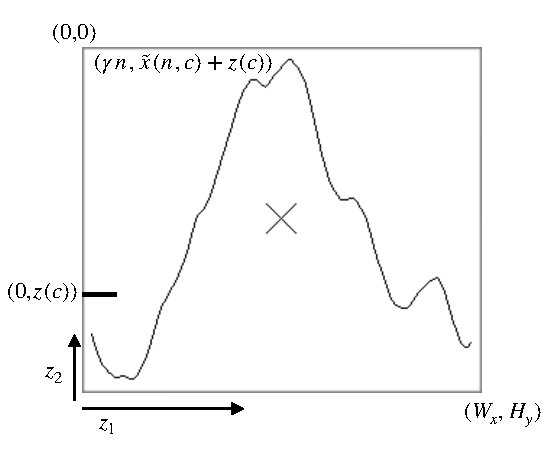
\includegraphics[scale=1]{images/imagecoordinatesystem.pdf}
\caption[Image Coordinate System]{A K-Complex transient event is shown on the image }
\label{fig:imagecoordinatesystem}
\end{figure}

\subsection{Pixelation}

EEG time-series are floating-point numbers and the image is constructed based on discrete and integer pixels.  To map one to the other you need to account for the rounding.

\begin{equation}
\tilde{x}(n,c) = \left \lfloor{ \gamma  \tilde{x}(n,c)  }\right \rceil
\label{eq:standarizedaverages}
\end{equation}

On the horizontal axis, $z_1$, no discretization is needed because time is already in sample units. 

\subsection{Interpolation}

Equation \ref{eq:images} produces a set of isolated pixels over the image.  To produce the plot $I^{(c)}$, the Bresenham \cite{Bresenham1965,Ramele2016} algorithm is used to interpolate straight lines between each pair of consecutive pixels.

Figure where the interpolation is shown.

However, as seen in Figure, it can lead to very sharp edges around the sample pixels.  This can lead to a quantization of histogram gradients, so another option is to use an interpolated version.  Instead of just skipping time points values, these values are interpolated according to a linear quadratic or cubic interpolation, which smooths the curve around each point.

Figure where the interpolation is improved.

(based on Matlab resample function) .resample applies an antialiasing FIR lowpass filter to x and compensates for the delay introduced by the filter.

Special care must be taken to avoid artifacts around the edges of the signal, so a window is also necessary to avoid this (like hamming).

\subsection{Resolution}

According to the plotting scheme, a resolution is established between pixel images and signal properties.

On the horizontal axis of the image, one pixel is equivalent to 

\begin{equation}
1 P_x \equiv \frac{1}{F_s \; \lambda \; \gamma_t}  [\si{s}]
\label{eq:resolutionx}
\end{equation}

\noindent where $F_s$ is the sampling frequency in Hertz, $\lambda$ is the span of the segment (in seconds), and $\gamma_t$ is the scale factor.  This gives a value in seconds.  For example, for Figure \ref{fig:imagecoordinatesystem}, the sampling frequency is $200 Hz$, the span is $0.65 s$ and $\gamma_t = 1$, which gives a resolution of $1 P_x \equiv 0.0077 s$. 

Consistently, on the vertical axis, one pixel is analogous to 

\begin{equation}
1 P_y \equiv \frac{1}{\gamma}  [\si\mu{V}]
\label{eq:resolutiony}
\end{equation}

\noindent where $\gamma$ is the signal scale.  As EEG time-series are digitalized in $\si\mu{V}$, this the unit of choice.  In Figure \ref{fig:imagecoordinatesystem}, $1$ vertical pixel represents exactly $1 \mu V$.
